\section{AG 3.2 - 8 - MAT - Himmelsrichtungen - OA - Matura 2019/20 1. HT}

\begin{beispiel}[AG 3.2]{1}
Nachstehend ist eine symmetrische Windrose abgebildet, die Himmeslrichtungen zeigt.

\begin{center}
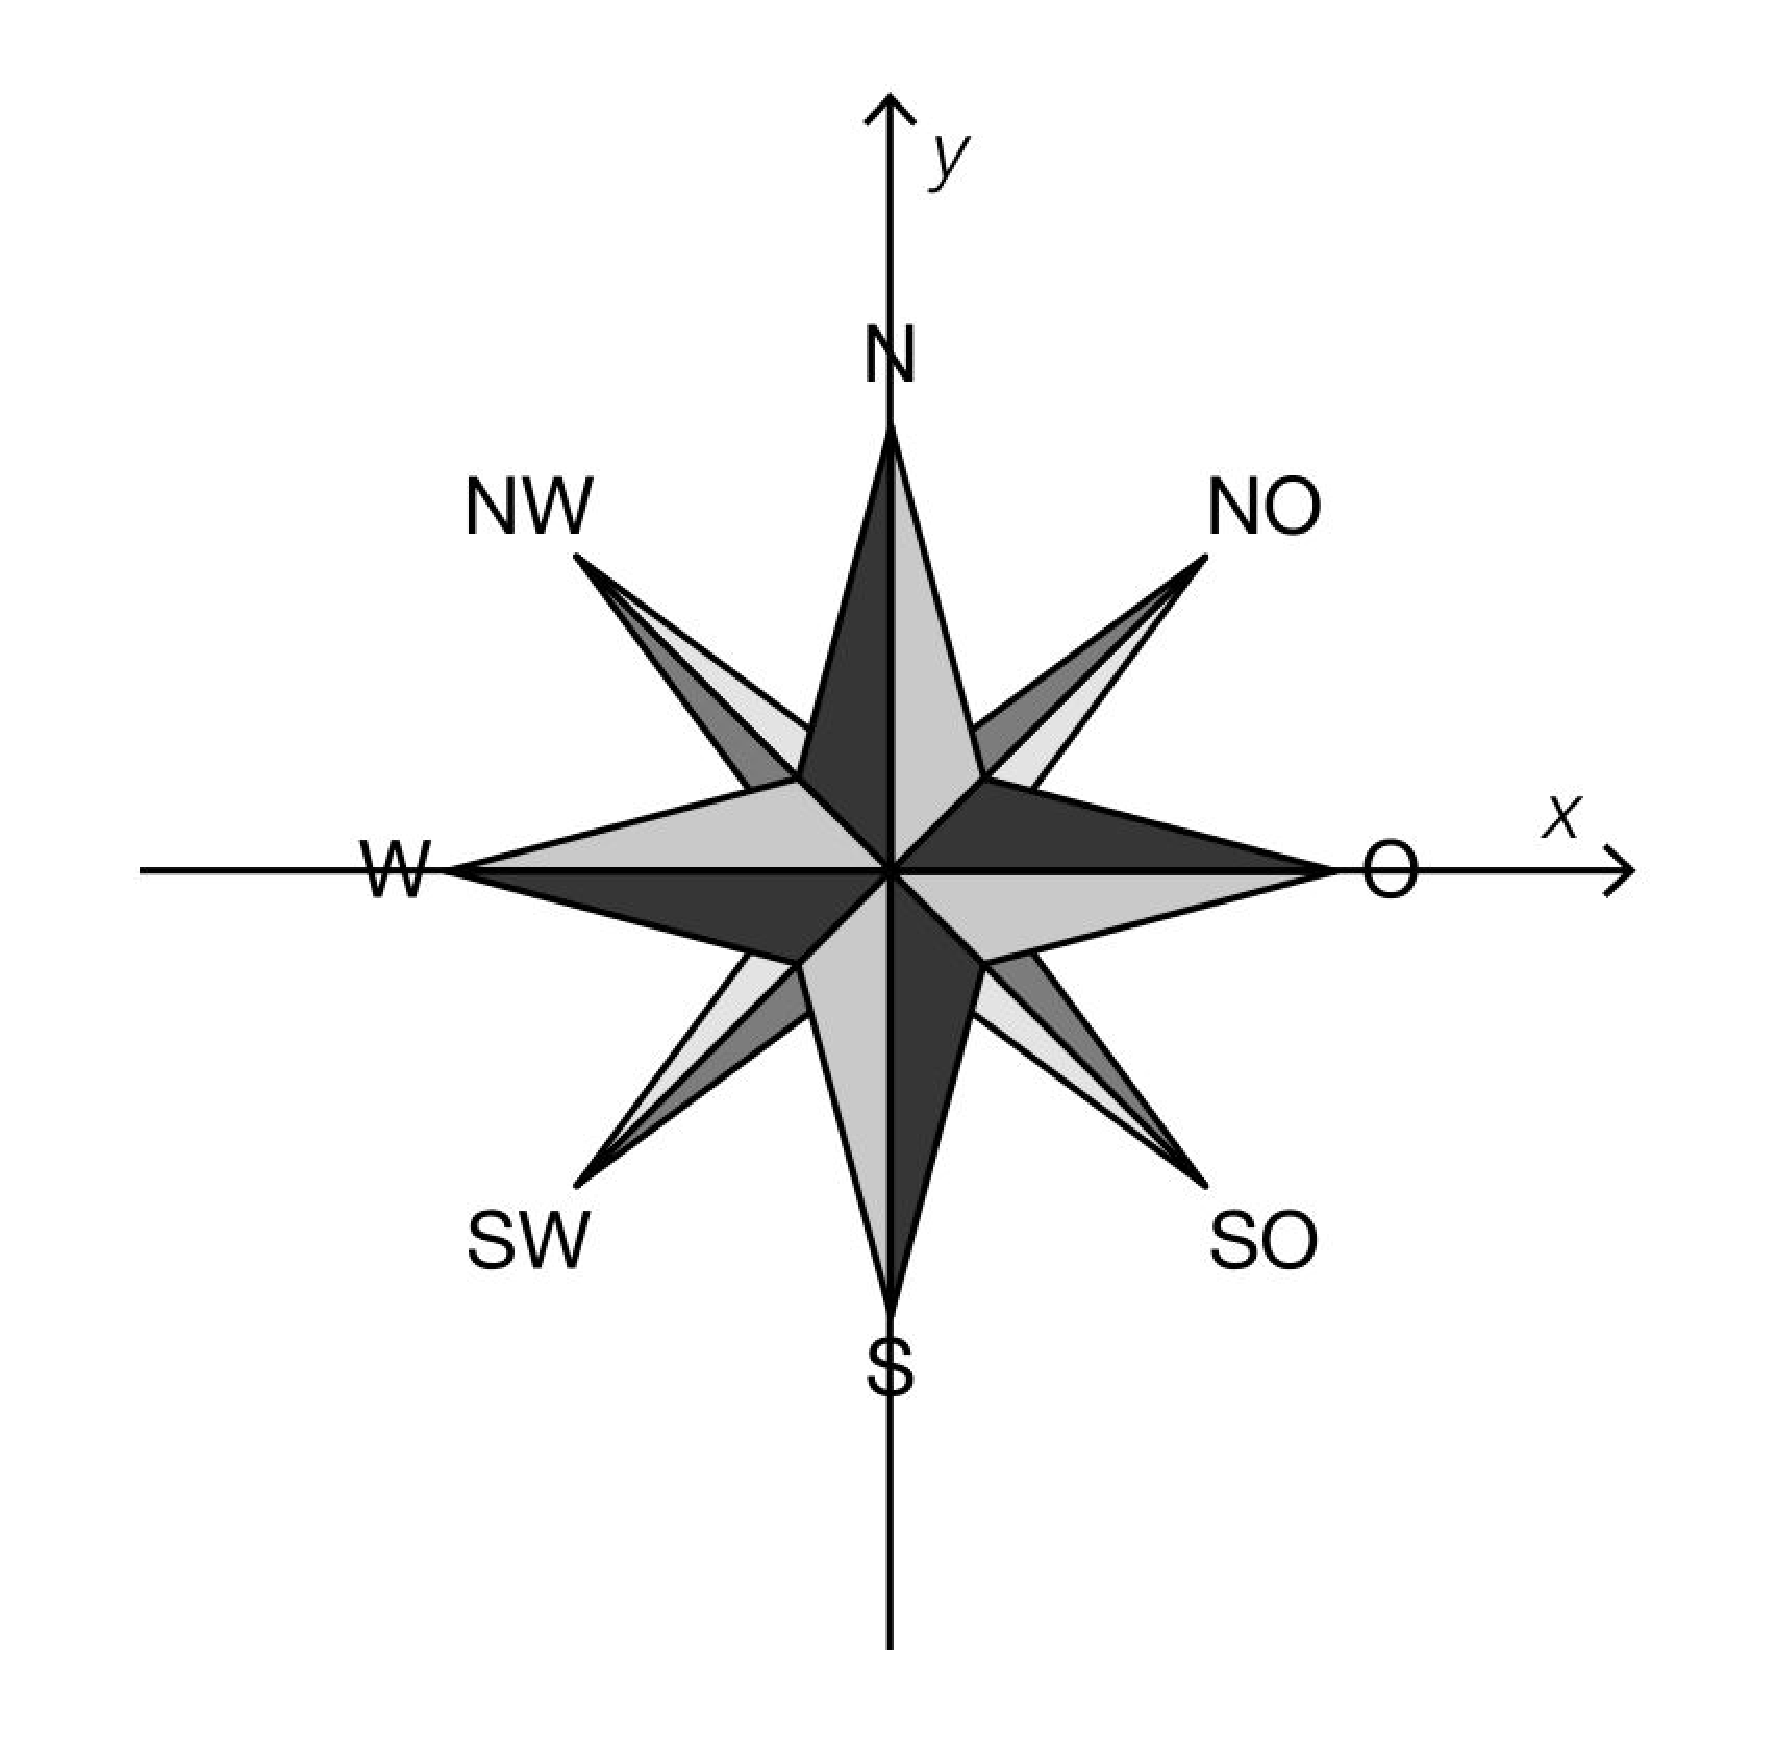
\includegraphics[width=0.5\textwidth]{../_database/Bilder/AG32_8_windrose.eps}
\end{center}

Die Geschwindigkeit eines Schiffes, das in Richtung Nordwest (NW) fährt, wird durch den Vektor $\vec{u}=\Vek{-a}{a}{}$ mit $a\in\mathbb{R}^+$ beschrieben.

Gib einen Vektor $\vec{v}$ an, der die Geschwindigkeit eines Schiffes beschreibt, das in Richtung Nordost (NO) fährt.\leer

$\vec{v}=\,\antwort[\rule{5cm}{0.3pt}]{\Vek{a}{a}{}}$

\antwort{Jeder Vektor $\vec{v}=r\cdot\Vek{a}{a}{}$ mit $r\in\mathbb{R}^+$ ist als richtig zu werten.}
\end{beispiel}